\chapter{Neutrino Identification: Finding MicroBooNE's first Neutrinos} \label{ch:neutrinoID}
The goal of the Neutrino Identification analysis was to positively identify BNB neutrino interactions in the MicroBooNE detector collected during the first days of running. Neutrino event candidates were identified in part by using a cut on detected flash of scintillation light during the 1.6 $\micro s$ beam-spill length of the BNB as well as identifying reconstructed object from the TPC that are neutrino like. After this selection, 2D and 3D event displays were used for verification of the selection performance. This selection was targeted to reduce the ratio of neutrino events to cosmic-only events from the initial 1 neutrino to 675 cosmics to a ratio of 1 to 0.5 or better which is equivalent to a background reduction by a factor of 1000 or more. These selected events were used for MicroBooNE's public displays of neutrino interactions. A clearly visible neutrino interaction with an identifiable vertex and at least 2 tracks originating from the vertex was what the analysis focused on. This analysis wasn't optimized for high purity or efficiency, but rather for very distinguishable neutrino interactions that could be identified by the public.
\section{Flash Finding}\label{sec:flashfinding}
Flash finding is the first step used in finding neutrino interactions. This section will detail how optical information is reconstructed as well as analysis scripts and event filters were used.
\subsection{Flash Reconstruction}
\begin{figure}[htp!]
\centering
	\begin{subfigure}[b]{.6\textwidth}
	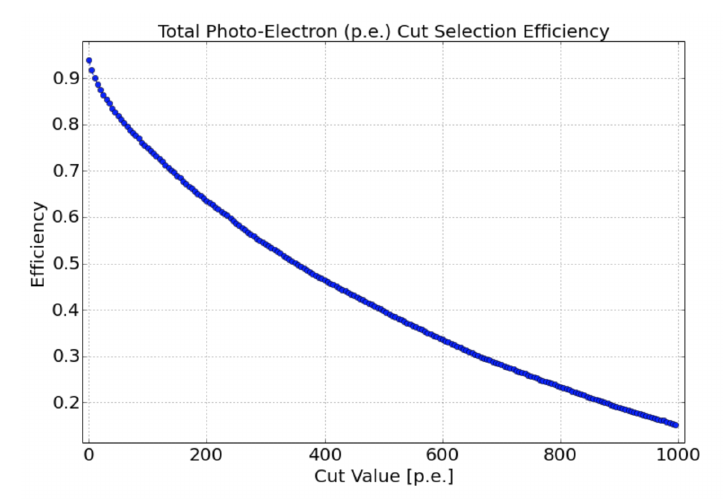
\includegraphics[width=\textwidth]{figs/totalpecut.png}
	\end{subfigure}
	\quad
	\begin{subfigure}[b]{.6\textwidth}
	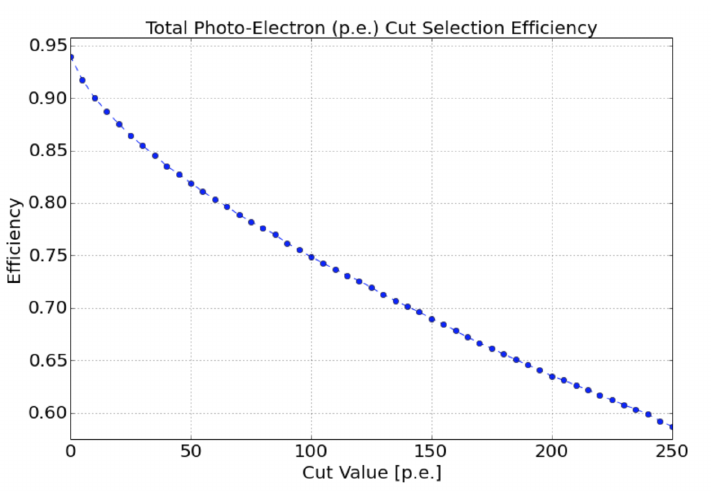
\includegraphics[width=\textwidth]{figs/totalpe_zoomed.png}
	\end{subfigure}
	\quad
\caption{Efficiency for selecting beam events as a function of minimum total PE cut for all PE cuts as well as zoomed into interesting region.}
\label{fig:PE}
\end{figure}
A flash is described as a collection of light seen at the same time within the detector. They are then reconstructed by identifying signal from the PMTs above a specific photoelectron (PE) threshold. These signals are called optical hits. Optical hits from all the PMTs are then accumulated into 1 $\micro s$ bins of time. If a specific bin is above a set PE threshold, then the optical hits that overlap in time are the labeled as the hits from the flash. All flash reconstructed properties like average time and x/y positions are then found via the flash labeled optical hits. The total size of the flash is found by summing up the total number of photoelectrons from all PMTs. Neutrino interactions and cosmic muons will have a larger flash size compared to noise and other low-energy backgrounds, therefore a total PE cut is used to reject these backgrounds. A total PE cut of 50 PE was deemed sufficient for this analysis. Figure \ref{fig:PE} show the total PE versus the selection efficency of selecting neutrino beam events. 


\subsection{Beam Timing}
\begin{figure}[htp!]
\centering
	\begin{subfigure}[b]{.6\textwidth}
	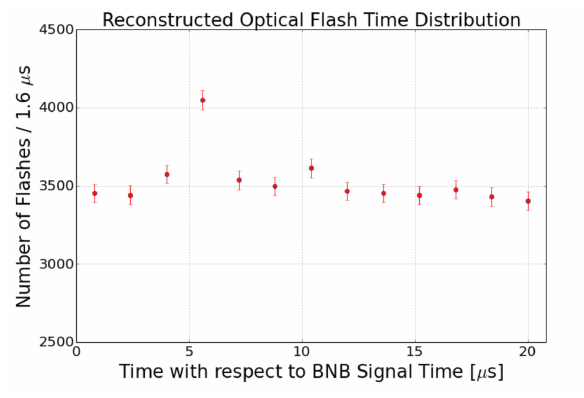
\includegraphics[width=\textwidth]{figs/flashrate_sim.png}
	\caption{Predicted distribution of flash times with respect to trigger time for 1 day of data taking at nominal rate and intensity}
	\label{fig:pe_sim}
	\end{subfigure}
	\quad
	\begin{subfigure}[b]{.6\textwidth}
	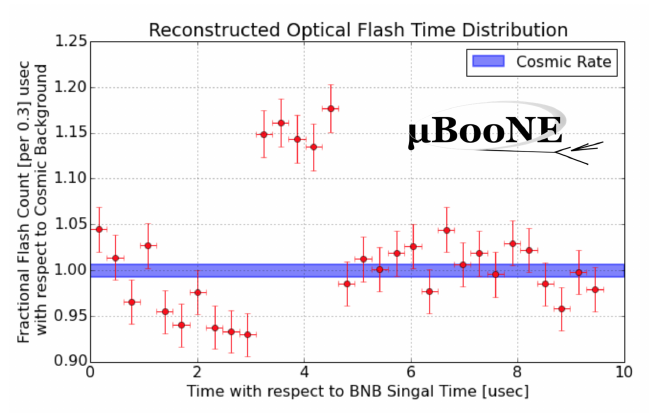
\includegraphics[width=\textwidth]{figs/flashrate.png}
	\caption{Measured distribution of flash times with a 50 PE threshold cut, with respect to trigger time. Shown as a ratio to the expected cosmic rate from off-beam data. A clear excess from neutrinos is visible between 3- 5 $\micro s$ after the trigger time. }
	\label{fig:pe_data}
	\end{subfigure}
	\quad
\label{fig:petime}
\end{figure}
It is necessary to get the specific time from flashes if one uses flashes to filter out neutrino interactions coincident with the neutrino beam spill period and background. Before a filter can be applied, an understanding of the timing of the trigger and PMT readout with respect to the arrival of neutrinos from the BNB. To do this, a 1.6 $\micro s$ window near the expected beamtime was created and verified by finding that the number of flashes was significantly above the cosmic-ray background flashes. Beam data during the first week of running, October 16th 2016 through October 22nd 2016 and were used for a timing measurement. The total POT uses corresponds to roughly 24 hours of data taking at nominal intensity ($4 X 10^{12} ppp$) and a 5 Hz repetition rate. Figure \ref{fig:pe_sim} shows size of the expected neutrino signal in time using Monte Carlo predictions and figure \ref{fig:pe_data} shows the neutrino signal in data. The intensity in data is lower, however there can still be seen a significan excess above data.

\subsection{Event Rates}
Applying a 50 PE threshold cut inside a 1.6 $\micro s$ window reduces the cosmic-ray passing rate to 0.8\%. With a 5 Hz beam rate, this corresponds to 135 cosmics passing per hour. The neutrino passing rate for this filter is about 22 events per hour. To further increase the neutrino to cosmic ratio, TPC topology cuts were implemented and will be discussed in the following section.
\section{TPC Topology Selection}  
In order to further reduce the background of cosmic events, two independent selection streams using TPC wire data reconstruction was implemented. The first using 2D reconstructed clusters, and the second using 3D resonctructed tracks.
